\documentclass[12pt]{article}
\usepackage[a4paper,margin=1in,showframe]{geometry}
\usepackage{tikz}
\usetikzlibrary{
  chains,
  shapes.multipart,
  arrows.meta % supersedes the arrows library
}
\begin{document}
\begin{figure}[!ht]
\centering
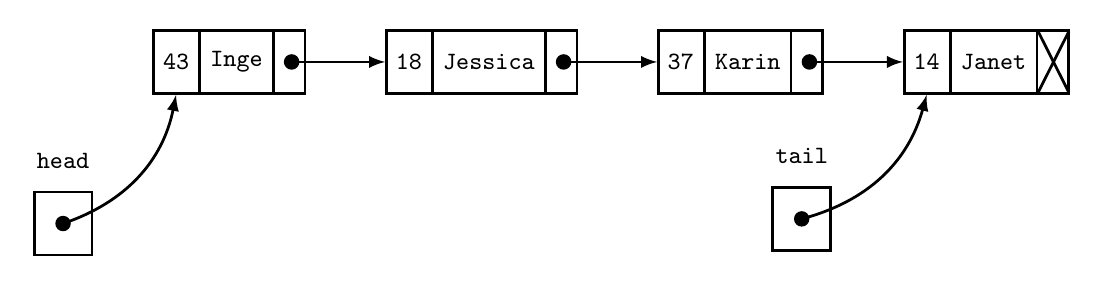
\begin{tikzpicture}[
  line width=1pt,
  font=\small\ttfamily,
  list/.style={
     rectangle split,
     rectangle split parts=3,
     draw,
     rectangle split horizontal,
%     minimum width=10cm,
     minimum height=.8cm,
  },
  headtail/.style={
     rectangle,
     draw,
     minimum height=.8cm
  },
  dotarrow/.style={Circle-latex},
  start chain
]
   % The nodes on the chain except for tail
   \node[on chain] (dummy) {};
   \node[list,on chain] (A) {43 \nodepart{two} Inge}; 
   \node[list,on chain] (B) {18 \nodepart{two} Jessica};
   \node[list,on chain] (C) {37 \nodepart{two} Karin};
   \node[list,on chain] (D) {14 \nodepart{two} Janet};
   \node[headtail,below=of C.three,yshift=-.5cm] (tail) {\phantom{tai}};
   \node[headtail,below=of dummy,yshift=-0.5cm] (head) {\phantom{tai}};
   
   % The null-pointer cross
   \draw[line cap=round, shorten >=.6pt, shorten <=.99pt] (D.north east) -- (D.two split south);
   \draw[line cap=round, shorten >=.6pt, shorten <=.99pt]  (D.south east) -- (D.two split north);
   
   % The connecting arrows
   \draw[dotarrow] (A.three |- A.center) -- (B);
   \draw[dotarrow] (B.three |- B.center) -- (C);
   \draw[dotarrow] (C.three |- C.center) -- (D);
%   \draw[-latex] (head.center |- A.center) -- (A);
   \draw[-latex] (head.center) to[bend right] (A.one south);
   \draw[fill=black] (head.center) circle (0.08);
   \draw[-latex] (tail.center) to[bend right] (D.one south);
   \draw[fill=black] (tail.center) circle (0.08);

   \node[yshift=0.8cm] at (tail.center) {tail};
   \node[yshift=0.8cm] at (head.center) {head};
   % the to path below extends the bounding box a lot, this fixes that
%   \useasboundingbox ([shift={(-1.3cm,0)}]A.north west) rectangle ([shift={(1cm,-7mm)}]D.south east);
%   \draw[dotarrow] (D.two |- D.center) to[out=-10,in=190,distance=6cm] (A);
\end{tikzpicture}
\caption{A linked list with four nodes with head and tail pointers.}
\end{figure}
\end{document} 